\documentclass[main]{subfiles}

\begin{document}

\section{How concurrency is achieved: Processes and Threads}
\subsection{Disclaimer}
% Make reference to useful learning materials such as Herlihy, Sophormic Intro and lecture slides/exercises
In this chapter, we want to explore the setting of the course. The final goal of the course is two-fold:\\
On the one hand, we want to be able to write multi-threaded programs in Java. But we also want to understand general concepts of concurrent programming and how to solve issues that arise with its introduction.\\
To get there, we first have to understand what a thread even is, how Java threads relate to them and how concurrency is achieved on the OS level.\\
Hence, before we start writing programs and analyze problems in concurrent programming, we take a look at how a modern OS handles programs and then define the setting the course takes place in. Note that this chapter explains multiprocessing in more depth than the course itself. It is not directly exam relevant, but the understanding gained in this chapter will be critical for later topics. At the end of the chapter, there is a short list of terms that are mentioned, but not explicitly explained in the text. When a term is not clear, it may be contained and explained in this list.
% sources: Thread states in Java: https://docs.oracle.com/javase/8/docs/api/java/lang/Thread.State.html
% Thread states and diagram: https://www3.ntu.edu.sg/home/ehchua/programming/java/j5e_multithreading.html
% os basics: processes, threads: https://web.archive.org/web/20201004050736/http://pages.cs.wisc.edu/~remzi/OSTEP/cpu-intro.pdf

\subsection{Threads and Processes from the OS Perspective}
A modern computer can run hundreds of programs at the same time with only a few cores. The operating system sits between these programs and the hardware and is responsible for making this work. On a high level, the OS first needs some way of organising these programs to get them ready for execution. It can then run a program for a bit, stop it, run another for a bit and so forth, creating the illusion of many programs running at the same time. We look at how this is achieved in more detail and discuss some important concepts.
\subsubsection{What is a process? [1]}
To start, we take a look at the lifecycle of a running program. Before the program is started, it is just a liveless collection of bits that sits on disk.\\
When we now start this program, the OS will make it come to live and view it as a \textit{process}. To achieve this, the OS loads the code and static data of the program from disk to main memory.
\begin{figure}[H]
    \centering
    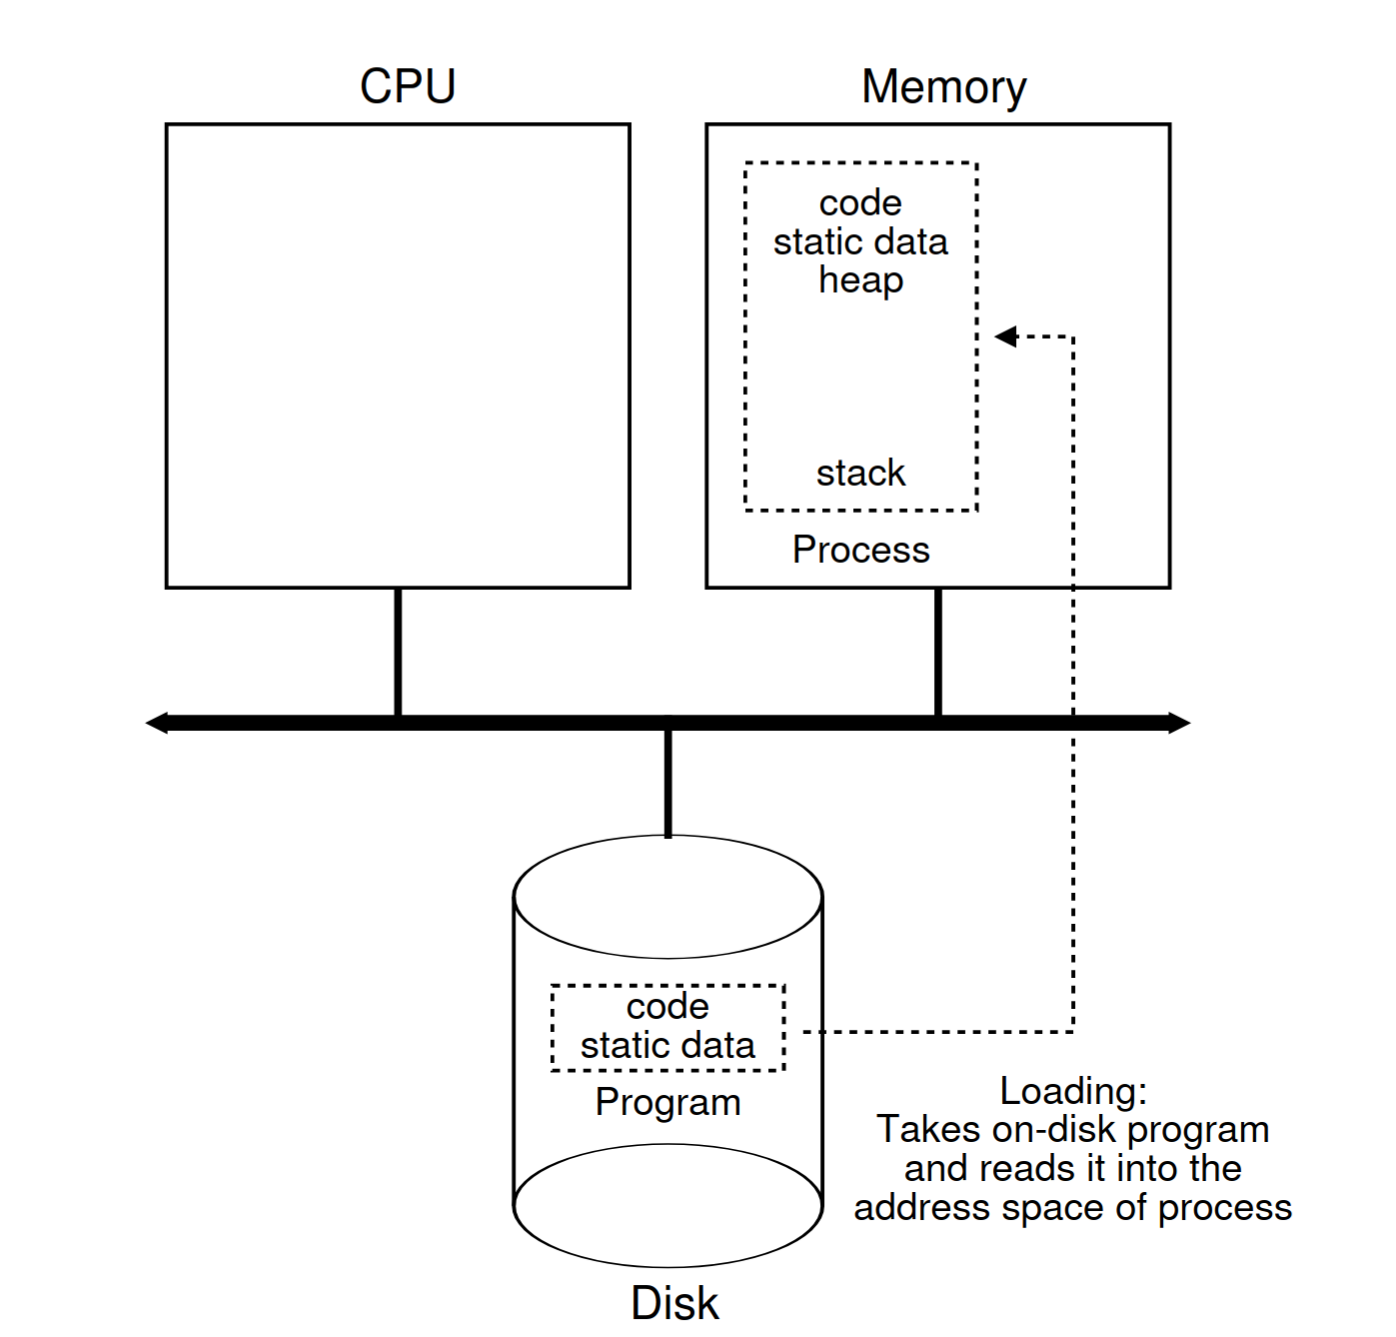
\includegraphics[scale=0.2]{ProgramToProcess.png}
    \caption{Program to Process. https://web.archive.org/web/20210627072431/https://pages.cs.wisc.edu/
    $\sim$remzi/Classes/537/Spring2018/Book/cpu-intro.pdf}
\end{figure}
To actually execute its code, the process also needs memory to store variables and data structures. Hence, the OS initializes an address space for the process and allocates a stack and usually also a heap within this address space. Allocating here simply means that the OS reserves a chunk of memory and tells the process where it is by passing pointers. Initializing an address space means that each process will \texttt{only} see its own memory locations. It cannot access memory of other processes.\\[3mm]
The OS also needs to do some other initialization related to I/O, such that the program can for example read and write to a console or deal with files.\\[3mm]
Going back to the beginning, we had a bunch of programs on disk we wanted to run at the same time. We transformed each of these programs into a process that has all the resources it requires to run loaded into main memory.
The OS views each running program now as a \textit{process} with an associated \textit{context} or \textit{state}, which includes all the things we mentioned before, like its address space, I/O information and CPU register state.\\[3mm]
All we need to do now is choose one process and start executing its code on the CPU.

\subsubsection{What is a thread now?}
Most operating systems further divide processes into threads. Further dividing the work of a process makes sense, as large programs have many different tasks that need to be taken care of at the same time. If we think of a running Java program, we need for example a garbage collector running in the background. \\[3mm]
In an OS that supports threads, each process consists of at least one thread and all threads within the same process share the same address space, that is, can view the same memory. This means that threads of the same process can easily communicate with each other, for example through shared variables. It also means that a thread has less \textit{context} it needs to store than a process. This is because it inherits most of its state from the parent process, like the address space and I/O information. We can think of threads as smaller processes:
\begin{figure}[H]
    \centering
    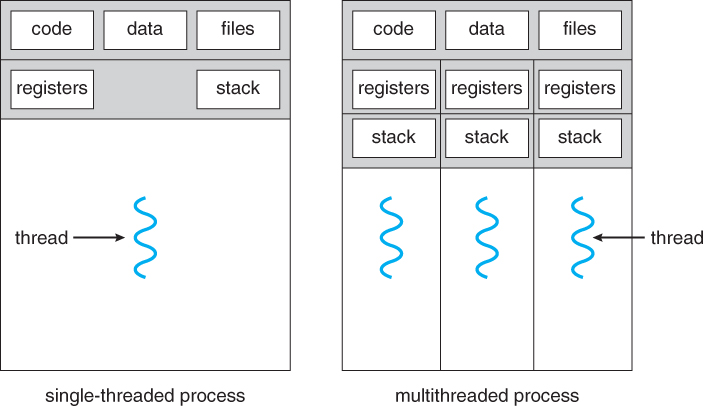
\includegraphics[scale=0.9]{ProcessAndThreads.jpg}
    \caption{Process vs. Thread. https://www.baeldung.com/cs/process-vs-thread}
\end{figure}

\subsubsection{Scheduling and Context Switches}
By introducing these OS concepts, the notion of parallelism boils down to how the OS divides the CPU cores on the competing processes and threads. \\
Imagine we have an n-core CPU. The OS can decide which process (and which of its threads) is running on each core at any time. The part of the OS responsible for this decision is referred to as the \textit{CPU scheduler} or just \textit{scheduler}. We can view the scheduler as a black box and just assume that it does a good job at giving sufficient CPU time to all processes and threads.\\
% Scheduling is done in three granularities:
% \begin{itemize}
%     \item \textit{Long-term scheduling}: Determines if the program is admitted to the system for processing. Decision happens when the thread is created.
%     \item \textit{Medium-term scheduling}: Decides which of the active processes are in main memory at any given time. Can swap out processes from main memory to secondary memory (usually disk).
%     \item \textit{Short-term scheduling}: Concerns which process (and which thread within the process) currently loaded into memory gets CPU access time.
% \end{itemize}
% We are concerned only with short-term scheduling in this course and whenever scheduling is mentioned, short-term scheduling is meant.
We assume a \textit{pre-emptive scheduler}, which just means that the scheduler can interrupt a thread at any time and swap it out for another thread, even if the thread didn't finish executing all its instructions yet.\\[3mm]
Descheduling a thread in favour of another is called a \texttt{context switch}. Upon a context switch, the OS has to store the context of the descheduled thread to memory and load the context of the newly scheduled thread from memory to the CPU core the thread is going to run on. Context switching threads is faster than context switching processes, but since a (thread) context switch is not meaningful work (as opposed to executing instructions of a running program), the OS still wants to minimize them.\\[3mm]
Imagine we have a process with three threads and only a single CPU core. Only a single thread can be scheduled at a time, as illustrated here:
\begin{figure}[H]
    \centering
    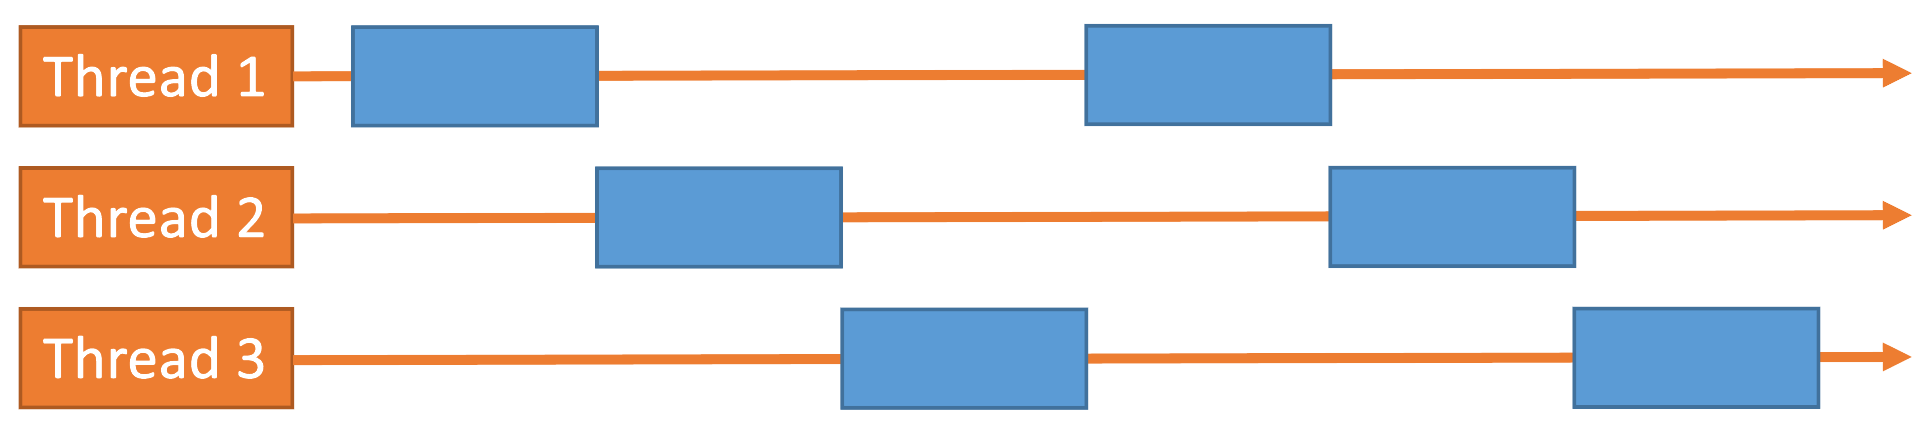
\includegraphics[scale=0.15]{ShareCPU.png}
    \caption{Multiple threads context switching on one core.}
\end{figure}
When we now have three CPU cores, all of these can be scheduled in parallel. For this to happen, the scheduler first has to schedule the process of the Java program on all three cores (remember, processes \textit{and} threads are scheduled). Then, all threads can run in parallel on separate cores:
\begin{figure}[H]
    \centering
    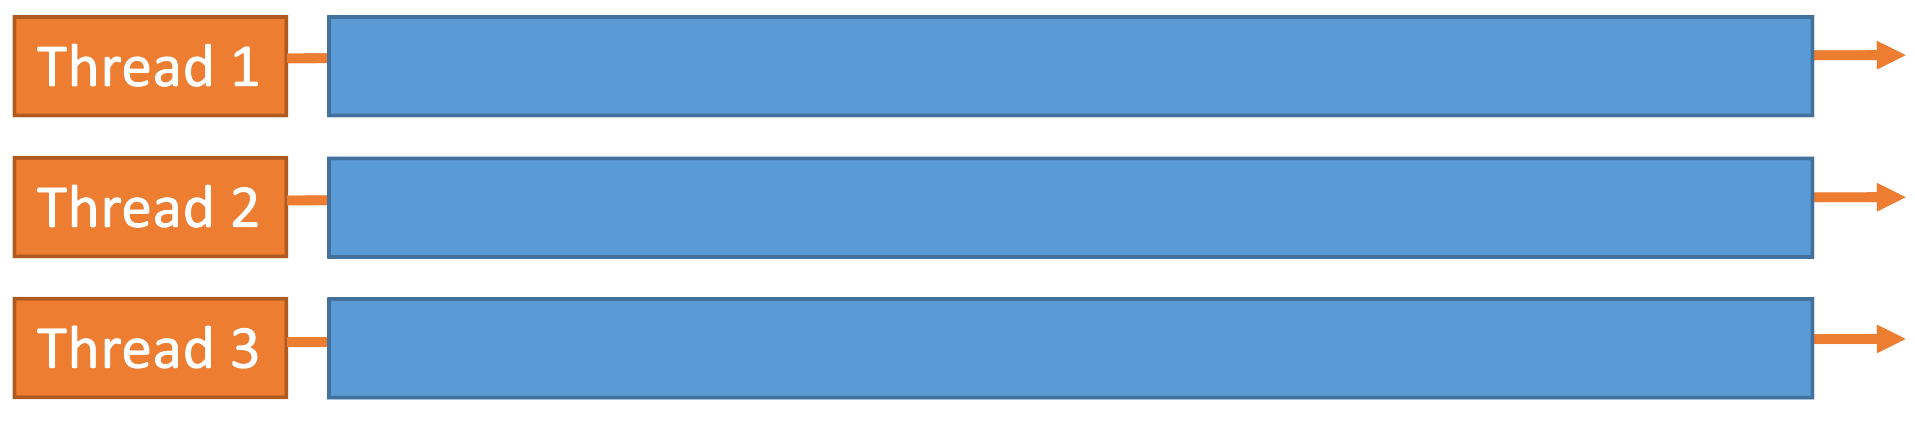
\includegraphics[scale=0.15]{SeparateCPU.png}
    \caption{Each thread runs on a separate core.}
\end{figure}
To context switch, we need to store everything a thread requires to continue executing its code later on. We now know how such a context switch can work: Since a thread inherits the address space from its parent process, it only needs to remember the CPU register contents. Note that the CPU registers include special registers like the instruction pointer and the stack pointer. Imagine we now switch out the thread for another (within the same process) and then switch back. Simply restoring these registers is enough to continue its execution with the next instruction, since the thread has the variables both on its stack and in the registers back and knows which instruction to execute next (since stack pointer, instruction pointer and other registers are restored). Note that the exact set of steps needed for such a switch depends on the OS, but generally, this is what is required.\\[3mm]
However, switching to a thread within another process is not as straightforward and we need to context switch to the other process first. Remember here that process context switching is a lot slower than thread context switching.

% \subsubsection{When does a thread get descheduled?}
% A thread might get descheduled when:
% \begin{itemize}
%   \item A more important thread needs CPU time. For example when a keyboard input is registered, the respective thread quickly requires CPU access and some other thread will need to get descheduled.
%   \item The thread accesses memory. Since a memory access can take millions of cycles, keeping this thread scheduled while it just waits for the data to arrive from memory is inefficient.
%         \item The threads CPU time sim
% \end{itemize}

\subsubsection{Concurrency vs Parallelism}
When two threads are now scheduled at the same time on different cores, they are executing in \textit{parallel}. However, we say that two threads are running \textit{concurrently}, when their lifetimes overlap. Two threads can run concurrently without ever being scheduled at the same time.\\
It is easy to show this on a single-core CPU. Imagine the OS only has two threads and keeps context switching between them. These threads run concurrently without ever actually executing instructions at the same time.\\[3mm]
Imagine a scenario again with two threads and a single core. The OS can decide to schedule the first thread until it completes and dies. It then schedules the second thread until it completes its tasks and dies. Even though the actual execution time of the first and second thread do not overlap, we still say that they run \textit{concurrently}, because their lifetime overlaps (the second thread was \textit{runnable}, but not scheduled while the first thread was scheduled). We see that concurrency is more of a conceptual property of a program; multiple tasks/threads are order-independent and \textit{can} be run in parallel.\\[3mm]
On a high level, we could say that concurrency is about \textit{dealing} with multiple things at the same time, while parallelism is about \textit{doing} these things at the same time.


% \subsection{\textit{Digression}: Why does my CPU claim 4 cores and 8 threads? Simultaneous Multi-Threading}
% On some PC's specification sheet n cores and 2n threads are listed. We also say that there are 2n logical cores. To the OS, the CPU appears to have 2n cores, meaning that it can schedule 2n threads at the same time. To understand this, we first need to understand that modern CPU's are pipelined.\\
% We imagine a simplified CPU with 5 pipeline stages: Fetching, decoding, operand fetching, computation and write-back. In each clock cycle, a new instruction is fetched and each instruction already in the pipeline moves on to the next stage, except when the operands of any instruction are not available yet (dependencies in the code). In this case, all instructions before that one in the pipeline are stalled until the operands are available.\\
% Consider the two toy programs A and B, which are compiled to the following machine code:
% \\A:
% \begin{minted}[]{gas}
% MOV $0 %eax          // A1: %eax <- 0
% ADD %eax %eax        // A2: %eax <- %eax + %eax
% \end{minted}
% B:
% \begin{minted}[]{gas}
% XOR %ebx %ebx        // B1: %ebx <- %ebx XOR %ebx
% ADD $5 %ecx          // B2: %ecx <- %ecx + 5
% MUL %ebx %ebx        // B3: %ebx = %ebx x %ebx
% \end{minted}
% We label the instructions A1, A2 and B1, B2, B3. Because of dependencies in the programs, both A and B have to stall the pipeline once and the overall execution takes 12 cycles when first fetching A1, A2, then B1, B2, B3. In practice, between A2 and B1 a context switch happens from thread A to thread B, which takes many cycles to complete, since all register values of thread A have to be loaded to memory and the context of thread B has to be loaded from memory.\\
% Now assume we have an Intel CPU supporting Intel's SMT implementation called Hyperthreading. In this case, there are two copies of all registers, one for each thread. Hence, both thread A and B have their context saved in registers at the same time. Now, the CPU can decide in each cycle whether to fetch the next instruction of thread A or thread B. Whenever a dependence occurs, the CPU can just fetch an instruction of the other thread instead of stalling the pipeline. In our toy example, this will look like this:\\
% The two advantages of SMT are that:
% \begin{enumerate}
%     \item Less context switches are required, since multiple thread contexts can be loaded into each core at the same time.
%     \item The pipeline has to stall less, since we can fetch independent instructions of another thread whenever dependencies or memory accesses occur.
% \end{enumerate}
% Most modern Intel CPU's implement SMT by providing twice the amount of registers per CPU core, such that two threads can be running concurrently without context switching. From above example, it should be clear that this approach does not give a 2x speedup. However, it is effective at decreasing so-called bubbles in the pipeline and hence maximizing resource usage.
%
% To conclude, the OS can treat such a system as having 2n cores, since it can schedule 2n OS threads at any given point in time. Note that the factor of 2 is well-chosen, but could also be any other positive integer m, as long as there are m copies of the architectural registers in each core.
%
\subsection{Java Threads}
The concept of a thread exists in multiple layers of abstraction. What we talked about so far are threads on the OS level. These are used as a means of organising running programs on the system.\\[3mm]
Programs themselves can also expose threads to the programmer. In many languages, these are so-called \textit{virtual threads} or \textit{green threads} and have to be treated as an additional level of abstraction, since they are managed by the language itself and not the OS.\\
In Java however, the thread library exposed by the language is very closely related to actual OS threads, since user created threads are 1-to-1 mapped to OS threads. This is called \textit{native threading}. Technically, the JVM specification does not specify a Java thread to OS thread mapping, but all current JVM implementations use such a 1-to-1 mapping.\\
Thus, we can talk about Java threads on the same abstraction level we did so far. Every executing program in Java is made up of threads. Even a normal single-threaded Java program runs on the \textit{main thread}.\\
We can imagine a Java thread as a sequence of [machine] instructions that are executed sequentially. Keep in mind that the machine will execute machine instructions compiled from your Java code and not your Java code itself.

\subsubsection{Creating Java Threads}
We demonstrate three viable methods of creating Java threads from within a Java program. When starting such an object, the JVM will tell the OS to create a new thread within the process of the running Java program. Appreciate that now its run method will be executing concurrently to the main thread in its own OS thread.
\begin{enumerate}
    \item Create a custom class implementing the runnable interface.
    \begin{minted}[]{java}
    public class MyRunnable implements Runnable {
        @Override
        public void run() {
            /* write code to be executed upon
            starting the thread here
            */
        }
    }
    \end{minted}
    Now we can instantiate this class in our code, construct a Thread instance with it and have its run method execute concurrently on another thread:
    \begin{minted}[]{java}
    MyRunnable r = new MyRunnable();
    Thread t = new Thread(r);
    t.start(); // starts t and executes its run() method
    \end{minted}
    We start a thread by calling start() on an object instance. Note that we can also execute the run() method of a Runnable or Thread by simply doing a function call:
    \begin{minted}[]{java}
    MyRunnable r = new MyRunnable();
    Thread t = new Thread(r);
    t.run(); // usually not what we want
    \end{minted}
    This executes the run method on the same thread instead of creating a new one and is usually not what we want.
    Keep in mind that this is a normal Java class and we could add other methods, fields and constructors.
    The only limitation is that the run method cannot return anything. We can get around that with shared variables (remember, threads within the same process see the same memory).

    \item Extend the Java Thread class:
    \begin{minted}[]{java}
    public class MyThread extends Thread {
        @Override
        public void run() {
            /* write code to be executed upon
            starting the thread here
            */
        }
    }
    \end{minted}
    Note that using this method, our MyThread class cannot extend another class, while using the first method this would be possible.\\
    We can now instantiate the MyThread class and start the instantiation.
    \begin{minted}[]{java}
    MyThread t = new MyThread();
    t.start(); // starts t and executes its run() method
    \end{minted}

    \item The most compact method is to create the code that is run by the thread anonymously and inline:
    \begin{minted}[]{java}
    Thread t = new Thread() {
        @Override
        public void run() {
            /* write code to be executed upon
            starting the thread here
            */
        }
    };
    t.start();
    \end{minted}
\end{enumerate}

\subsubsection{Daemon vs Non-Daemon Threads}
Java differentiates daemon threads that are responsible for background tasks like memory management (for example the garbage collector is a daemon thread) and non-daemon threads, which execute the program itself. The main thread is non-daemon and so are all user-created threads by default.\\
A Java program only terminates once all non-daemon threads die. This means in particular that non-daemon threads can continue to run, even when the main() method returned.\\
User-created threads are non-daemon by default. In this course, we will exclusively work with non-daemon threads.

\subsubsection{Setting of this course}
In this course, we analyze multi-threaded [Java] programs. Where is such a program now located in the context of this chapter?\\
First of all, we are always on a single machine. This course does not cover \textit{distributed} systems consisting of more than one machine. However, the machine we assume usually has multiple cores.\\
We are usually within a single process (the process of our executing Java program). When we talk about context switches, we usually mean switching from one Java thread to another. But we are also mindful that the system can schedule other processes and threads in between.\\
We are almost always talking about non-daemon threads, that is, the main thread and user-created threads. Our Java threads can run in parallel on different cores, but also concurrently on the same core. This is all decided by the scheduler and out of our control.

% \subsubsection{Thread states [2]}
% If we want to be able to talk about the effects of different thread operations, we need some notion of \textit{thread states}. In short, a Java thread typically goes through the following states:
% \begin{itemize}
%     \item \textit{New}: Once the \texttt{Thread} object is created, the thread enters the new state. At this point, the thread is just an object in the heap and no resources have been allocated for it.
%     \item \textit{Runnable}: Once we call \texttt{start()} on the new thread object, the system allocates resources to enable its execution and the thread becomes eligible for being scheduled.
%     \item \textit{Running}: When the thread is actually scheduled to run.
%     \item \textit{Not runnable}: We use this as an umbrella state for multiple states that cause the thread to not be runnable. The thread enters this state when one of the following events occur:
%         \begin{enumerate}
%             \item The sleep() method is called to suspend the thread for a specified amount of time to yield control to the other threads.
%             \item The wait() method is called to wait for a specific condition to be satisfied.
%             \item The thread is blocked and waiting for an I/O operation to be completed. Attempting to acquire a lock and calling join() will also cause a thread to be blocked, but these two topics will be covered later on.
%         \end{enumerate}
%     These methods and terms will be covered in the next chapter. At this point we just note that even though our Java threads are scheduled by the OS, we still have \textit{some} control over them from the language itself.
%     \item \textit{Terminated}: A thread transitions to terminated state when the run() method terminates and exits.
% \end{itemize}
% \begin{figure}[H]
%     \centering
%     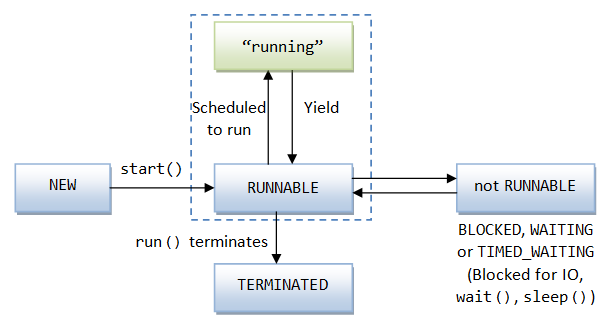
\includegraphics[scale=0.8]{ThreadLifeCycle.png}
% \end{figure}
% There is a getState() method in Java returning one of the states \textit{new}, \textit{runnable}, \textit{blocked}, \textit{waiting}, \textit{timed waiting} and \textit{terminated}:
% \begin{minted}[]{java}
% Thread T = new Thread() {
%     public void run() {
%         System.out.println(Thread.currentThread().getState());
%     }
% };
% T.start();

% > RUNNABLE // prints the state to the console
% \end{minted}
% We notice that Java differentiates some states we simply put into a \textit{not runnable} state. Later in the script we are going to introduce additional concepts related to these states and mention the state diagram again.

\subsection{Summary}
What is important to remember from this section is that threads are primarily a unit of organization for the OS and are what ultimately runs on the CPU. Their lightweight nature is what enables the scheduler to quickly swap them in and out of the CPU and thus creating the illusion of many programs running at the same time. Although Java threads are created by the JVM rather than the OS, they are (usually) 1-to-1 mapped to OS threads and hence we can think about them the same way.

\subsection{What is/are again...}
\begin{itemize}
  \item ...\textit{CPU registers}? Registers are a small set (usually about 8-32) of memory locations directly on a CPU core. We cannot access them in a high-level programming language. They are used by the compiler for local variables, as compared to data structures, which are usually placed in the heap. Since registers are directly on the CPU core, they are orders of magnitude faster to access than main memory and even caches.\\
  The registers used for storing variables are referred to as \textit{general purpose registers}. There are also some special registers, like the instruction pointer (stores the memory address of the instruction to be executed next) and stack pointer (stores the memory address of the top of the stack).
  \item ...\textit{the heap}? The heap is a contiguous memory region in main memory. Each process has its own heap and uses it for storing datastructures. If you create an array or an object in your Java code, it will be stored on the heap when the program runs. The heap is actively managed by the system to make sure the space is efficiently used.
  \item ...\textit{the stack}? The stack is also a contiguous memory region in main memory. Usually, each thread within a process has its own stack. It is not actively managed by the system and thus faster to allocate and deallocate memory from than the heap. The compiler usually puts variables on the stack when all registers are already used.
  \item ...\textit{an address space}? We mentioned that each process has its own address space. What does this mean? To access a memory location, a process does not use the actual \textit{physical} address, but instead a \textit{virtual} address. We can imagine a virtual layer on top of the memory locations. Each virtual address gets mapped to a physical location when it is used. This means that different processes use a different \textit{virtual} address to refer to the same \textit{physical} address. The advantage of this is that for each process, we can simply slap a virtual layer on top of the memory addresses and to the process it will appear that the memory is empty, since its virtual addresses are not mapped yet. This is why a process cannot access another process' memory: It simply cannot see it.\\
  This whole concept is known as \textit{virtual memory} and it not part of this course. Just know that when we say a new process gets its own address space, it means that the OS initializes a new empty virtual layer to be filled by the process.
    \begin{figure}[H]
        \centering
        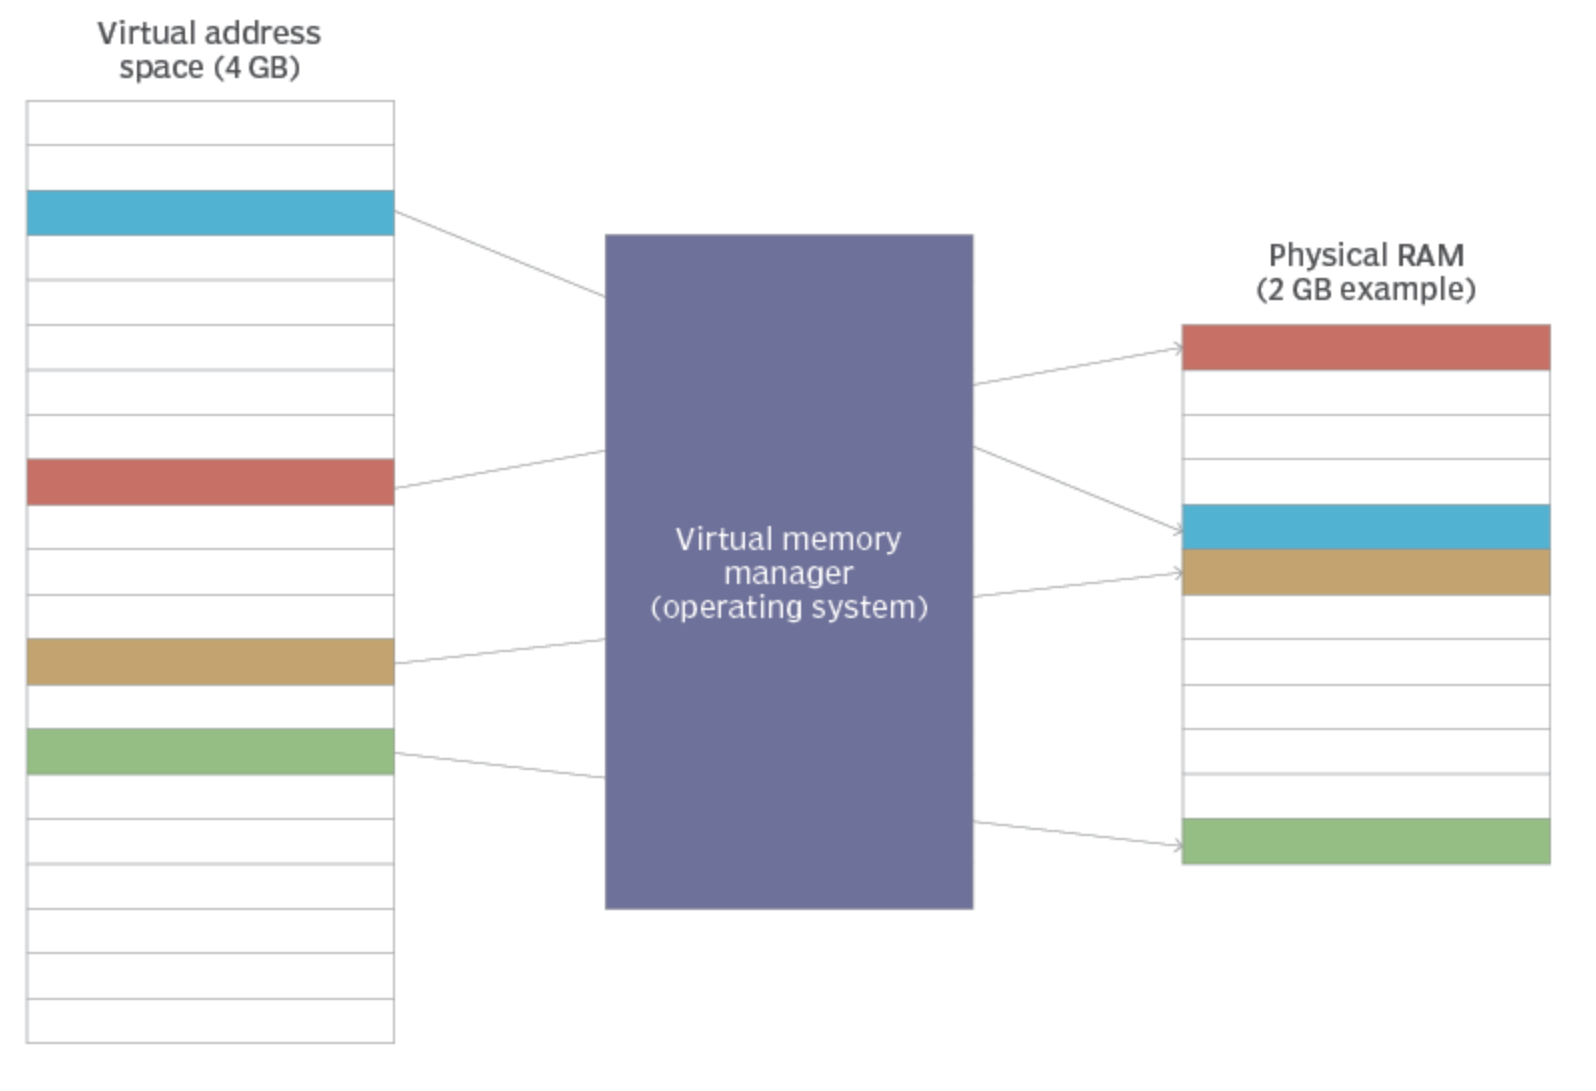
\includegraphics[scale=0.2]{VirtualMem.png}
        \caption{Virtual to Physical Address Mapping. https://www.techtarget.com/whatis/definition/virtual-address}
    \end{figure}

\end{itemize}

\subsection{References}
[1]: Operating Systems: Three Easy Pieces: Chapter 4; The Abstraction: The Process. Available at: https://web.archive.org/web/20201004050736/http://pages.cs.wisc.edu/~remzi/OSTEP/cpu-intro.pdf.
% [2]: https://www3.ntu.edu.sg/home/ehchua/programming/java/j5e_multithreading.html

% TODO:
% - Add Java methods for controlling threads: Sleep, interrupt, join... also then explain how they relate to the state model
% - Maybe first give some more intuition on how to use threads with examples.
% - find a diagram for SMT to add a digression section`'
% - incorporate last slide of L03-05: Summary of thread states


% \subsection{Bad Interleavings and Data Races}
% A \textit{race condition} is a mistake in your program such that whether the program behaves correctly or not depends on the order in which the threads execute. Race conditions are very common bugs in concurrent programming that, by definition, do not exist in sequential programming. We distinguish two types of race conditions.\\[3mm]
% One kind of race condition is a \textit{bad interleaving}. The key point is that ''what is a bad interleaving'' depends entirely on what you are trying to do. Whether or not it is okay to interleave two bank-account withdraw operations depends on some specification of how a bank is supposed to behave.
% \begin{example}
%     Suppose we have the following implementation of a \texttt{peek} operation on a concurrent stack.
%     \begin{figure}[H]
%         \centering
%         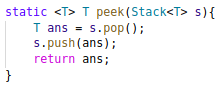
\includegraphics[scale=0.45]{peekWrong.png}
%     \end{figure}
%     \noindent Assume that the \texttt{pop} and \texttt{push} methods are implemented correctly. While \texttt{peek} might look like it's implemented correctly, the following interleaving might occur:
%     \begin{figure}[H]
%         \centering
%         \begin{subfigure}{.5\textwidth}
%             \centering
%             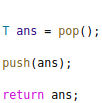
\includegraphics[scale=0.45]{BadInterleaving_1.png}
%             \captionsetup{labelformat=empty}
%             \caption{Thread 1 (\texttt{peek)}}
%         \end{subfigure}%
%         \begin{subfigure}{.5\textwidth}
%             \centering
%             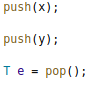
\includegraphics[scale=0.45]{BadInterleaving_2.png}
%             \captionsetup{labelformat=empty}
%             \caption{Thread 2}
%         \end{subfigure}
%     \end{figure}
% \end{example}
% A \textit{data race} is a specific kind of race condition that is better described as a ''simultaneous access error'', although nobody uses that term. There are two kinds of data races:
% \begin{itemize}
%     \item When one thread might read an object field at the same moment that another thread writes the same field.
%     \item When one thread might write an object field at the same moment that another thread also writes the same field.
% \end{itemize}
% \noindent Notice it is not an error for two threads to both read the same object field at the same time.\\[3mm]
% Our programs must never have data races even if it looks like a data race would not cause an error - if our program has data races, the execution of your program is allowed to do very strange things: The exact behavior that the program is allowed to exhibit is usually defined in the memory model of a language, we'll get to the memory model of Java later.
% \begin{example}
%     Let's consider a very simple example.
%     \begin{figure}[H]
%         \centering
%         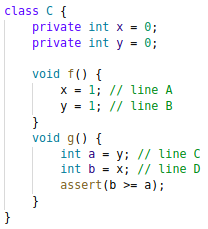
\includegraphics[scale=0.45]{DataRace.png}
%     \end{figure}
%     Notice that \texttt{f} and \texttt{g} are not synchronized, leading to potential data races on fields \texttt{x} and \texttt{y}, Therefore, the assertion in \texttt{g} can fail. But there is no interleaving of operations that justifies the assertion failure, as can be seen through a proof by contradiction: \\[3mm]
%     \quad Assume the assertion fails, meaning \texttt{!(b$>=$a)}. Then \texttt{a==1} and \texttt{b==0}. Since \texttt{a==1}, line B happened before line C. Since A must happen before B, C must happen before D, and ''happens before'' is a transitive relation, A must happen before D. But then \texttt{b==1} and the assertion holds.\\[3mm]
%     There is nothing wrong with the proof except its assumption that we can reason in terms of ''all possible interleavings'' or that everything happens in certain orders. We can reason this way only if the program has no data races.
% \end{example}
%
% \subsection{Other Models}
% We've introduced a programming model of explicit threads with shared memory. This is, of course, not the only programming model for concurrent or parallel programming. Shared memory is often considered convenient because communication uses ''regular'' reads and writes of object fields. However, it's also considered error-prone because communication is implicit; it requires a deep understanding of the code/documentation to know which memory accesses are doing inter-thread communication and which are not. The definition of shared-memory programs is also much more subtle than many programmers think because of issues regarding data races, as discussed in the previous section.\\[3mm]
% Three well-known, popular alternatives to shared memory are presented in the following. Note that different models are better suited for different problems. Models can be abstracted and freely built on top of each other or we can use multiple models in the same program (e.g. MPI with Java).\\[3mm]
% \textit{Message-passing} is the natural alternative to shared memory. In this model, explicit threads do not share objects. For them to communicate, copies of data are exchanged as messages between processes. As objects are not shared between individual threads, the issue of threads wrongly updating fields does not occur. One does, however, have to keep track of the different data copies being passed around through messages. Message passing is especially fitting for processes which are far apart form each other, similar to sending an email, where a copy of the message is sent to the recipient.\\[3mm]
% \textit{Dataflow} provides more structure than having ''a bunch of threads that communicate with each other however they want.'' Instead, the programmer uses primitives to create a directed acyclic graph. A node in the graph performs some computation using inputs that arrive on its incoming edges. This data is provided by other nodes along their outgoing edges. A node starts its computation when all of its inputs are available, something the implementation keeps track of automatically.\\[3mm]
% \textit{Data parallelism} does not have explicit threads or nodes running different parts of the program at different times. Instead, it has primitives for parallelism that involve applying the same operation to different pieces of data at the same time. For example, you would have a primitive for applying some function to every element of an array. The implementation of this primitive would use parallelism rather than a sequential for-loop. Hence all the parallelism is done for you provided you can express your program using the available primitives.
%
\end{document}
